\begin{figure}[t!]
	\centering
	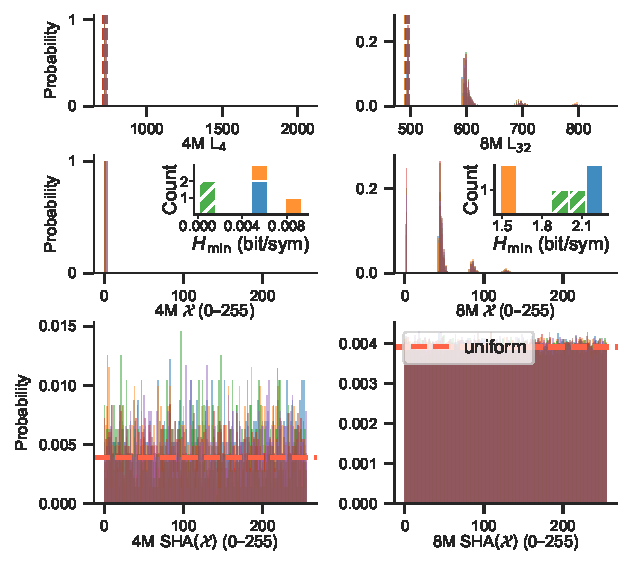
\includegraphics[width=0.9\linewidth]{img/trng_flow_RST_sidebyside.pdf}
	\caption{
		Raw samples (top), symbol mappings and per-region Hmin (middle), and conditioned output (bottom) for 4 fresh 4M (left) and 4 fresh 8M (right) 256B test regions. The $H_{min}$ of each region is colored according the chip in which the region is locate. Two regions are measured at 50\textdegree~C are colored green with a striped texture. NIST 90b reports extremely low $H_{min}$ for all tested regions in the 4M modules, making the required data collection for the NIST-22 and PractRand impractical, while the 8M performs extremely well.
		\label{fig:eval-entropy}
	}
\end{figure}